\documentclass[11pt,a4paper]{article}

% ============================================================================
% Packages
% ============================================================================
\usepackage[utf8]{inputenc}
\usepackage[T1]{fontenc}
\usepackage{times}
\usepackage[margin=1in]{geometry}
\usepackage{graphicx}
\usepackage{booktabs}
\usepackage{amsmath,amssymb}
\usepackage{multirow}
\usepackage{caption}
\usepackage{subcaption}
\usepackage{hyperref}
\usepackage{xcolor}
\usepackage{float}
\usepackage{enumitem}
\usepackage{natbib}
\usepackage{fancyhdr}

% ============================================================================
% Document Settings
% ============================================================================
\hypersetup{
    colorlinks=true,
    linkcolor=blue,
    citecolor=blue,
    urlcolor=blue
}

\captionsetup{font=small,labelfont=bf}
\setlength{\parindent}{0.5cm}
\setlength{\parskip}{0.3em}

\pagestyle{fancy}
\fancyhf{}
\rhead{Self-Supervised Learning for Medical OOD Detection}
\lhead{}
\rfoot{Page \thepage}

% ============================================================================
% Title
% ============================================================================
\title{
\textbf{Self-Supervised Learning for Out-of-Distribution Detection in Medical Imaging: A Comparative Study of JEPA, MAE, and Supervised Learning}
}

\author{
% Add your name and affiliation here
}

\date{\today}

% ============================================================================
% Document
% ============================================================================
\begin{document}

\maketitle

% ============================================================================
% Abstract
% ============================================================================
\begin{abstract}
Out-of-distribution (OOD) detection is a critical capability for the safe deployment of machine learning models in medical imaging, where systems inevitably encounter data from diverse sources that differ from the training distribution. This study presents a comprehensive comparative analysis of three representation learning paradigms---Joint Embedding Predictive Architecture (JEPA), Masked Autoencoder (MAE), and supervised learning---for chest X-ray out-of-distribution detection. Using the TB Chest Radiography Database as in-distribution data and the Montgomery and Shenzhen tuberculosis datasets as out-of-distribution test sets, we evaluate OOD detection performance, cross-dataset generalization, and robustness to common image corruptions. Our experimental results demonstrate that self-supervised methods significantly outperform supervised learning on energy-based OOD detection, achieving 77-87\% AUROC compared to 58-61\% for supervised approaches. Furthermore, MAE exhibits exceptional robustness to contrast perturbations, maintaining 98.3\% classification AUC under severe corruption where JEPA and supervised methods degrade to 67-76\%. Mahalanobis distance-based detection achieves near-perfect performance (95-99\% AUROC) across all methods, suggesting that distribution-aware scoring can compensate for representation differences. These findings provide practical guidance for deploying medical imaging AI systems with reliable OOD detection capabilities, with extensions to echocardiogram segmentation proposed as future work.
\end{abstract}

\textbf{Keywords:} Out-of-Distribution Detection, Self-Supervised Learning, Medical Imaging, Chest X-ray, JEPA, Masked Autoencoder, Vision Transformer

% ============================================================================
% 1. Introduction
% ============================================================================
\section{Introduction}

The deployment of deep learning models in medical imaging has demonstrated remarkable success across various diagnostic tasks, including disease classification, lesion detection, and anatomical segmentation \citep{litjens2017survey}. However, a fundamental challenge persists: medical imaging systems in clinical practice inevitably encounter data that differs from the training distribution. These out-of-distribution (OOD) samples may arise from variations in imaging equipment, acquisition protocols, patient demographics, or pathological presentations not represented in the training data \citep{castro2020causality}. When models encounter such distributional shifts, they often produce overconfident yet incorrect predictions, posing significant risks to patient safety and clinical decision-making \citep{kompa2021second}.

Reliable OOD detection is therefore essential for trustworthy medical AI deployment. An effective OOD detection system should identify when input data differs substantially from the training distribution, enabling appropriate human oversight or abstention from automated predictions. Traditional approaches to OOD detection, including confidence-based methods \citep{hendrycks2017baseline} and density estimation techniques \citep{ren2019likelihood}, have shown limited effectiveness when applied to high-dimensional medical images with subtle distributional shifts.

Self-supervised learning (SSL) has emerged as a promising paradigm for learning robust visual representations without requiring labeled data \citep{chen2020simple, he2020momentum}. By designing pretext tasks that exploit the inherent structure of visual data, SSL methods can learn features that capture semantic content while being invariant to superficial variations. Recent architectures such as the Joint Embedding Predictive Architecture (JEPA) \citep{assran2023self} and Masked Autoencoders (MAE) \citep{he2022masked} represent two distinct approaches to self-supervised representation learning. JEPA predicts latent representations of masked image regions, hypothesized to capture high-level semantic features, while MAE reconstructs pixel-level content, potentially learning more fine-grained visual patterns.

Despite the theoretical promise of self-supervised representations for OOD detection, their practical effectiveness in medical imaging remains understudied. Medical imaging presents unique challenges for OOD detection: datasets are typically small, class imbalances are common, and the distribution shifts of clinical interest (e.g., different hospital equipment) may be subtle compared to natural image domain shifts.

This work presents a systematic comparison of JEPA, MAE, and supervised pretraining for chest X-ray OOD detection. Our contributions are as follows:

\begin{enumerate}[leftmargin=*]
    \item We provide a comprehensive evaluation of three representation learning paradigms (JEPA, MAE, supervised) using standardized architectures and training protocols, enabling fair comparison.
    
    \item We evaluate OOD detection using multiple scoring functions (energy score, Mahalanobis distance) across two clinically relevant OOD datasets from different hospital sources.
    
    \item We analyze cross-dataset generalization and robustness to common image corruptions (noise, blur, contrast shifts), revealing significant differences between pretraining approaches.
    
    \item We identify practical recommendations for deploying medical imaging systems with reliable OOD detection, highlighting MAE's superior robustness and the effectiveness of Mahalanobis-based scoring.
\end{enumerate}

% ============================================================================
% 2. Related Work
% ============================================================================
\section{Related Work}

\subsection{Out-of-Distribution Detection}

Out-of-distribution detection has received substantial attention in the machine learning community, with methods broadly categorized into confidence-based, density-based, and distance-based approaches.

\textbf{Confidence-based methods} leverage the observation that neural networks tend to produce lower confidence predictions on OOD samples. The seminal work by \citet{hendrycks2017baseline} proposed using the maximum softmax probability as an OOD score, establishing a simple yet effective baseline. Subsequent work introduced temperature scaling \citep{guo2017calibration} and input perturbation techniques \citep{liang2018enhancing} to improve separation between in-distribution and OOD samples. \citet{liu2020energy} proposed energy-based OOD detection, demonstrating that the energy function $E(\mathbf{x}) = -\log \sum_c \exp(f_c(\mathbf{x}))$ provides theoretically grounded and empirically superior OOD scores compared to softmax confidence.

\textbf{Density-based methods} attempt to model the distribution of in-distribution data explicitly. Likelihood-based generative models \citep{nalisnick2019deep} and normalizing flows \citep{kirichenko2020normalizing} have been explored for OOD detection, though \citet{ren2019likelihood} demonstrated that likelihood alone is insufficient, proposing likelihood ratios instead. Variational autoencoders with reconstruction-based scoring \citep{an2015variational} have also been applied to medical imaging OOD detection.

\textbf{Distance-based methods} measure the distance between test samples and the training distribution in feature space. The Mahalanobis distance approach \citep{lee2018simple} fits class-conditional Gaussian distributions to penultimate layer features and computes the minimum Mahalanobis distance to class centroids. This approach has proven particularly effective when combined with feature ensemble techniques across multiple layers.

In medical imaging, OOD detection has been studied for various modalities including chest X-rays \citep{cao2020benchmark}, fundus images \citep{band2021benchmarking}, and histopathology \citep{linmans2020efficient}. However, most prior work has focused on supervised representations, leaving the potential of self-supervised methods largely unexplored.

\subsection{Self-Supervised Learning in Vision}

Self-supervised learning has transformed visual representation learning by enabling training on unlabeled data through carefully designed pretext tasks.

\textbf{Contrastive methods} such as SimCLR \citep{chen2020simple} and MoCo \citep{he2020momentum} learn representations by maximizing agreement between differently augmented views of the same image while minimizing agreement with other images. These methods have achieved remarkable success on natural image benchmarks, with representations rivaling or exceeding supervised pretraining for downstream tasks. DINO \citep{caron2021emerging} and its successor DINOv2 \citep{oquab2024dinov2} extend this framework with self-distillation, learning particularly strong features for semantic segmentation and object detection.

\textbf{Masked image modeling} represents an alternative approach inspired by masked language modeling in NLP \citep{devlin2019bert}. The Masked Autoencoder (MAE) \citep{he2022masked} masks a large portion (75\%) of image patches and trains an encoder-decoder architecture to reconstruct the missing pixels. The asymmetric design, where only visible patches are processed by the encoder, enables efficient training while learning representations that capture both local and global image structure. BEiT \citep{bao2022beit} and SimMIM \citep{xie2022simmim} explore variations of masked image modeling with different reconstruction targets.

\textbf{Joint Embedding Predictive Architecture (JEPA)} \citep{assran2023self} represents a recent paradigm that predicts representations rather than pixels. Unlike MAE, which reconstructs raw pixel values, JEPA predicts the latent embeddings of target image regions from context regions. This approach avoids the pixel-level details that may be irrelevant for downstream tasks, instead focusing on learning semantic features. The architecture employs separate context and target encoders with exponential moving average (EMA) updates for the target encoder, similar to momentum-based contrastive methods.

\subsection{Self-Supervised Learning in Medical Imaging}

The application of self-supervised learning to medical imaging has gained significant momentum, driven by the scarcity of labeled data in clinical domains \citep{chen2019self, azizi2021big}.

\citet{sowrirajan2021moco} demonstrated that MoCo pretraining on chest X-rays improves downstream classification performance compared to ImageNet pretraining. \citet{azizi2021big} showed that contrastive pretraining with multi-instance learning achieves state-of-the-art results on dermatology and chest X-ray classification. More recently, foundation models pretrained on large medical imaging datasets \citep{huang2023foundation} have shown strong transfer learning capabilities.

For echocardiography, self-supervised methods have been applied to tasks including view classification \citep{dezaki2017cardiac}, quality assessment \citep{abdi2017automatic}, and cardiac function estimation \citep{ouyang2020video}. Video-based approaches leverage temporal consistency for self-supervision, though frame-level pretraining remains common for segmentation tasks.

Despite this progress, systematic comparisons of different self-supervised paradigms for medical OOD detection remain limited. Our work addresses this gap by providing a controlled comparison of JEPA, MAE, and supervised pretraining for chest X-ray OOD detection.

% ============================================================================
% 3. Methodology
% ============================================================================
\section{Methodology}

This section describes the self-supervised pretraining approaches, downstream evaluation protocols, and OOD detection methods employed in our study.

\subsection{Problem Formulation}

Let $\mathcal{D}_{\text{ID}} = \{(\mathbf{x}_i, y_i)\}_{i=1}^{N}$ denote the in-distribution dataset with images $\mathbf{x}_i$ and labels $y_i \in \{0, 1\}$ (Normal, Tuberculosis). We aim to learn an encoder $f_\theta: \mathcal{X} \rightarrow \mathbb{R}^d$ that produces representations suitable for both downstream classification and OOD detection. Given a trained encoder and linear classifier, OOD detection requires distinguishing samples from $\mathcal{D}_{\text{ID}}$ versus out-of-distribution datasets $\mathcal{D}_{\text{OOD}}$ representing different hospital sources.

\subsection{Architecture}

All experiments use the Vision Transformer Small (ViT-S) architecture \citep{dosovitskiy2021image} to ensure fair comparison across pretraining methods. The ViT-S encoder consists of 12 transformer blocks with embedding dimension 384, 6 attention heads, and MLP dimension 1536, totaling approximately 21.6 million parameters. Input images are resized to $224 \times 224$ pixels and divided into $16 \times 16$ patches, yielding 196 patch tokens plus a classification (CLS) token.

% Architecture Figure
\begin{figure}[t]
    \centering
    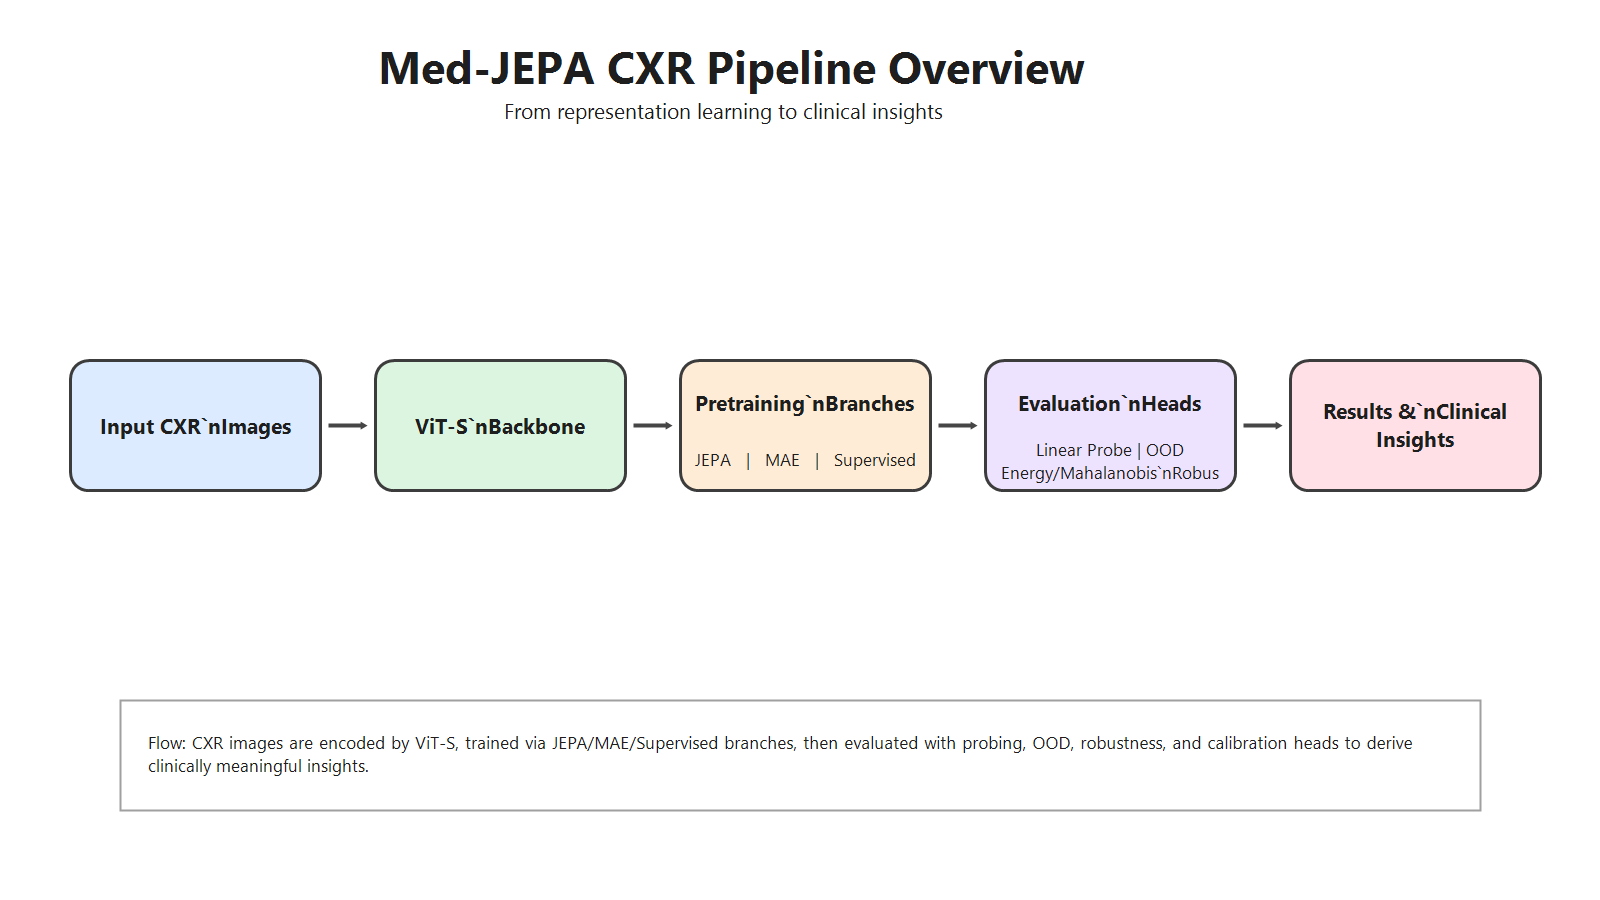
\includegraphics[width=\textwidth]{figures/architecture.png}
    \caption{\textbf{System Architecture Overview.} Medical images undergo self-supervised pretraining using JEPA, MAE, or supervised learning to train a ViT-Small encoder. The learned representations are evaluated through linear probing for classification, OOD detection using energy and Mahalanobis scores, and robustness testing under image corruptions.}
    \label{fig:architecture}
\end{figure}

\subsection{Self-Supervised Pretraining Methods}

\subsubsection{JEPA (Joint Embedding Predictive Architecture)}

JEPA learns representations by predicting target patch embeddings from context patches in latent space, rather than reconstructing pixel values. The architecture consists of three components:

\textbf{Context Encoder:} Processes visible (context) patches and produces representations $\mathbf{h}_{\text{ctx}} = f_\theta(\mathbf{x}_{\text{ctx}})$.

\textbf{Target Encoder:} An exponential moving average (EMA) copy of the context encoder that processes target patches: $\mathbf{h}_{\text{tgt}} = f_{\bar{\theta}}(\mathbf{x}_{\text{tgt}})$, where $\bar{\theta} \leftarrow \tau \bar{\theta} + (1-\tau) \theta$ with momentum $\tau \in [0.996, 1.0]$.

\textbf{Predictor:} A lightweight transformer that predicts target representations from context representations: $\hat{\mathbf{h}}_{\text{tgt}} = g_\phi(\mathbf{h}_{\text{ctx}}, \mathbf{m}_{\text{tgt}})$, where $\mathbf{m}_{\text{tgt}}$ are learnable mask tokens indicating target positions.

The training objective minimizes the $L_2$ distance between predicted and actual target representations:
\begin{equation}
    \mathcal{L}_{\text{JEPA}} = \frac{1}{|\mathcal{T}|} \sum_{t \in \mathcal{T}} \|\hat{\mathbf{h}}_t - \text{sg}(\mathbf{h}_t)\|_2^2
\end{equation}
where $\mathcal{T}$ denotes the set of target patches and $\text{sg}(\cdot)$ is the stop-gradient operation.

We use 85-100\% context masking with 4 target blocks of 15-20\% each, following \citet{assran2023self}. The predictor consists of 6 transformer blocks with embedding dimension 384.

\subsubsection{MAE (Masked Autoencoder)}

MAE learns representations through masked image reconstruction. The architecture uses an asymmetric encoder-decoder design:

\textbf{Encoder:} Processes only visible (unmasked) patches, reducing computational cost. With 75\% masking ratio, only 25\% of patches are encoded.

\textbf{Decoder:} A lightweight transformer that receives encoded visible patches and learnable mask tokens, reconstructing pixel values for all patches.

The training objective is mean squared error on normalized pixel values:
\begin{equation}
    \mathcal{L}_{\text{MAE}} = \frac{1}{|\mathcal{M}|} \sum_{m \in \mathcal{M}} \|\hat{\mathbf{p}}_m - \mathbf{p}_m\|_2^2
\end{equation}
where $\mathcal{M}$ denotes masked patch indices and $\mathbf{p}_m$ are patch pixel values normalized per-patch.

We use 75\% random masking following \citet{he2022masked}, with a decoder of 4 transformer blocks and embedding dimension 256.

\subsubsection{Supervised Pretraining}

The supervised baseline trains the ViT-S encoder end-to-end with a classification head using cross-entropy loss:
\begin{equation}
    \mathcal{L}_{\text{sup}} = -\sum_{i=1}^{N} \sum_{c=1}^{C} y_{i,c} \log \hat{y}_{i,c}
\end{equation}
where $\hat{y}_{i,c}$ are softmax probabilities from the classification head applied to the CLS token representation.

\subsection{Downstream Evaluation}

\subsubsection{Linear Probing}

For all pretrained encoders, we freeze the encoder weights and train a linear classifier on extracted features. The CLS token representation $\mathbf{z} = f_\theta(\mathbf{x})_{\text{[CLS]}} \in \mathbb{R}^{384}$ serves as the image-level embedding. A linear layer $\mathbf{W} \in \mathbb{R}^{2 \times 384}$ maps embeddings to class logits, trained with cross-entropy loss on the in-distribution training set.

\subsubsection{OOD Detection Methods}

\textbf{Energy Score} \citep{liu2020energy}: The energy function provides a scalar score indicating how well an input conforms to the learned data distribution:
\begin{equation}
    E(\mathbf{x}; T) = -T \cdot \log \sum_{c=1}^{C} \exp(f_c(\mathbf{x}) / T)
\end{equation}
where $f_c(\mathbf{x})$ are logits and $T$ is temperature. Lower energy indicates in-distribution samples. We use $T=1$ following standard practice.

\textbf{Mahalanobis Distance} \citep{lee2018simple}: This approach fits class-conditional Gaussian distributions to the embedding space. Given class means $\boldsymbol{\mu}_c$ and shared covariance $\boldsymbol{\Sigma}$, the Mahalanobis distance for a test embedding $\mathbf{z}$ is:
\begin{equation}
    M(\mathbf{z}) = \min_{c} \sqrt{(\mathbf{z} - \boldsymbol{\mu}_c)^\top \boldsymbol{\Sigma}^{-1} (\mathbf{z} - \boldsymbol{\mu}_c)}
\end{equation}
Higher distance indicates OOD samples. We estimate $\boldsymbol{\mu}_c$ and $\boldsymbol{\Sigma}$ from the in-distribution training set.

\subsection{Robustness Evaluation}

We evaluate robustness to common image corruptions that may occur in clinical settings:

\begin{itemize}[leftmargin=*]
    \item \textbf{Gaussian Noise:} Additive Gaussian noise with increasing variance, simulating sensor noise.
    \item \textbf{Gaussian Blur:} Convolution with Gaussian kernels of increasing size, simulating defocus.
    \item \textbf{Contrast Perturbation:} Multiplicative contrast adjustment, simulating exposure variations.
\end{itemize}

Each corruption is applied at 6 severity levels (0-5), where level 0 represents clean images. We report classification AUC at each severity level to assess degradation patterns.

% ============================================================================
% 4. Experiments and Results
% ============================================================================
\section{Experiments and Results}

\subsection{Experimental Setup}

\subsubsection{Datasets}

\textbf{In-Distribution (ID):} The TB Chest Radiography Database \citep{rahman2020reliable} contains 4,200 chest X-ray images with binary labels (Normal: 700 images, Tuberculosis: 3,500 images). We use an 80/20 train/validation split, resulting in 3,360 training and 840 validation samples.

\textbf{Out-of-Distribution (OOD):} We use two external tuberculosis datasets representing different hospital sources and imaging protocols:
\begin{itemize}[leftmargin=*]
    \item \textbf{Montgomery County TB Dataset} \citep{jaeger2014two}: 138 chest X-rays from Montgomery County, Maryland, USA, acquired on a Eureka stationary X-ray machine.
    \item \textbf{Shenzhen Hospital TB Dataset} \citep{jaeger2014two}: 662 chest X-rays from Shenzhen No.3 People's Hospital, Guangdong Province, China, acquired on a Philips DR Digital Diagnost system.
\end{itemize}

These OOD datasets represent realistic distribution shifts encountered when deploying models across different healthcare institutions.

\subsubsection{Implementation Details}

All models use ViT-Small architecture with identical hyperparameters for fair comparison. Pretraining runs for 50 epochs with batch size 32, AdamW optimizer with learning rate $5 \times 10^{-4}$ and cosine decay. Data augmentation is limited to random resized cropping (scale 0.3-1.0) without horizontal flipping to preserve anatomical consistency. Linear probes train for 100 epochs with learning rate $1 \times 10^{-3}$. All experiments use a single NVIDIA GPU with mixed-precision training.

\subsubsection{Evaluation Metrics}

\begin{itemize}[leftmargin=*]
    \item \textbf{Classification:} Area Under ROC Curve (AUROC), Accuracy
    \item \textbf{Calibration:} Expected Calibration Error (ECE), Negative Log-Likelihood (NLL)
    \item \textbf{OOD Detection:} AUROC (ID vs. OOD), False Positive Rate at 95\% True Positive Rate (FPR@95)
\end{itemize}

\subsection{In-Distribution Classification Performance}

Table \ref{tab:id_classification} presents classification performance on the in-distribution TB Database validation set.

\begin{table}[h]
\centering
\caption{\textbf{In-Distribution Classification Performance} on TB Chest Radiography Database (n=840). All methods achieve strong classification performance, with supervised learning showing slight advantages due to direct optimization for the classification objective.}
\label{tab:id_classification}
\begin{tabular}{@{}lcccc@{}}
\toprule
\textbf{Method} & \textbf{AUROC} & \textbf{Accuracy} & \textbf{ECE} & \textbf{NLL} \\
\midrule
JEPA & 0.939 & 0.917 & 0.029 & 0.206 \\
MAE & 0.993 & 0.971 & 0.013 & 0.085 \\
Supervised & \textbf{0.996} & \textbf{0.980} & \textbf{0.007} & \textbf{0.064} \\
\bottomrule
\end{tabular}
\end{table}

All three methods achieve strong in-distribution classification performance, with AUROC exceeding 0.93 across all approaches. Supervised learning achieves the highest performance (99.6\% AUROC), which is expected given direct optimization for the classification task. MAE closely follows (99.3\% AUROC), demonstrating that reconstruction-based pretraining learns highly discriminative features. JEPA shows somewhat lower ID performance (93.9\% AUROC), possibly due to its emphasis on predicting semantic features over fine-grained details relevant for TB detection.

Calibration metrics follow a similar pattern, with supervised learning showing the lowest expected calibration error (ECE = 0.007), indicating well-calibrated probability estimates on in-distribution data. These results establish that all pretrained representations capture task-relevant features, enabling subsequent analysis of OOD detection capabilities.

\subsection{OOD Detection Performance}

Tables \ref{tab:ood_energy} and \ref{tab:ood_mahal} present OOD detection results using energy score and Mahalanobis distance, respectively.

\begin{table}[h]
\centering
\caption{\textbf{OOD Detection with Energy Score.} Self-supervised methods (JEPA, MAE) substantially outperform supervised learning, particularly on the Shenzhen dataset where MAE achieves 86.6\% AUROC compared to 58.2\% for supervised.}
\label{tab:ood_energy}
\begin{tabular}{@{}lcccc@{}}
\toprule
& \multicolumn{2}{c}{\textbf{Montgomery}} & \multicolumn{2}{c}{\textbf{Shenzhen}} \\
\cmidrule(lr){2-3} \cmidrule(lr){4-5}
\textbf{Method} & \textbf{AUROC} & \textbf{FPR@95} & \textbf{AUROC} & \textbf{FPR@95} \\
\midrule
JEPA & \textbf{0.771} & \textbf{0.540} & 0.718 & 0.633 \\
MAE & 0.769 & 0.577 & \textbf{0.866} & \textbf{0.358} \\
Supervised & 0.607 & 0.814 & 0.582 & 0.931 \\
\bottomrule
\end{tabular}
\end{table}

Energy-based OOD detection reveals striking differences between pretraining paradigms. Self-supervised methods (JEPA and MAE) substantially outperform supervised learning on both OOD datasets. On the Montgomery dataset, JEPA and MAE achieve approximately 77\% AUROC compared to 61\% for supervised learning—a gap of 16 percentage points. The difference is even more pronounced on the Shenzhen dataset, where MAE achieves 86.6\% AUROC while supervised learning achieves only 58.2\%, barely above random chance.

This performance gap suggests that supervised representations overfit to discriminative features specific to the training distribution, resulting in unreliable confidence estimates for OOD samples. The supervised model's FPR@95 of 93.1\% on Shenzhen indicates that nearly all OOD samples are misclassified as in-distribution when requiring 95\% true positive rate—a dangerous failure mode for clinical deployment.

MAE demonstrates the strongest overall energy-based OOD detection, particularly on Shenzhen (86.6\% AUROC). This may be attributed to MAE's reconstruction objective, which requires modeling the full data distribution rather than just discriminative boundaries. JEPA shows competitive performance on Montgomery but lower performance on Shenzhen, suggesting the predicted semantic features may not fully capture distribution differences.

\begin{table}[h]
\centering
\caption{\textbf{OOD Detection with Mahalanobis Distance.} Distribution-aware scoring achieves excellent performance across all methods, with AUROC exceeding 95\% in most cases.}
\label{tab:ood_mahal}
\begin{tabular}{@{}lcccc@{}}
\toprule
& \multicolumn{2}{c}{\textbf{Montgomery}} & \multicolumn{2}{c}{\textbf{Shenzhen}} \\
\cmidrule(lr){2-3} \cmidrule(lr){4-5}
\textbf{Method} & \textbf{AUROC} & \textbf{FPR@95} & \textbf{AUROC} & \textbf{FPR@95} \\
\midrule
JEPA & 0.956 & 0.186 & 0.985 & 0.077 \\
MAE & \textbf{0.994} & \textbf{0.030} & 0.984 & 0.085 \\
Supervised & 0.991 & 0.024 & \textbf{0.997} & \textbf{0.000} \\
\bottomrule
\end{tabular}
\end{table}

Mahalanobis distance-based OOD detection achieves excellent performance across all methods, with AUROC exceeding 95\% in all cases. This contrasts sharply with energy-based detection, where supervised learning performed poorly. The Mahalanobis approach models the distribution of embeddings explicitly rather than relying on classifier confidence, effectively compensating for the limitations of discriminatively-trained representations.

Notably, supervised learning achieves the best Mahalanobis-based detection on Shenzhen (99.7\% AUROC with 0\% FPR@95), despite its poor energy-based performance. This suggests that supervised representations do capture distribution differences in embedding space, but these differences are not reflected in classifier confidence. MAE achieves the best performance on Montgomery (99.4\% AUROC), while JEPA shows slightly lower but still strong performance.

These results have important practical implications: combining supervised representations with Mahalanobis-based OOD scoring may provide reliable detection, though self-supervised methods offer more consistent performance across both scoring approaches.

\subsection{Cross-Dataset Generalization}

Table \ref{tab:cross_dataset} presents classification performance when linear probes trained on the ID dataset are evaluated on OOD datasets.

\begin{table}[h]
\centering
\caption{\textbf{Cross-Dataset Classification Generalization.} MAE demonstrates superior transfer to OOD datasets, suggesting reconstruction-based pretraining learns more generalizable features.}
\label{tab:cross_dataset}
\begin{tabular}{@{}lccc@{}}
\toprule
\textbf{Method} & \textbf{ID (AUC)} & \textbf{Montgomery (AUC)} & \textbf{Shenzhen (AUC)} \\
\midrule
JEPA & 0.992 & 0.554 & 0.430 \\
MAE & 0.995 & \textbf{0.607} & \textbf{0.695} \\
Supervised & \textbf{0.996} & 0.471 & 0.592 \\
\bottomrule
\end{tabular}
\end{table}

Cross-dataset transfer reveals MAE's superior generalization capabilities. While all methods achieve similar ID performance (99.2-99.6\% AUC), MAE significantly outperforms alternatives on OOD classification. On the Shenzhen dataset, MAE achieves 69.5\% AUC compared to 43.0\% for JEPA and 59.2\% for supervised—a 10-26 percentage point advantage.

JEPA shows unexpected behavior: despite strong ID performance, it transfers poorly to OOD datasets (43.0-55.4\% AUC, near random chance). This suggests that JEPA's predictive objective may encourage learning features specific to the training distribution's structure, which do not generalize across domain shifts. The masked prediction task may encode distribution-specific patterns in the context-target relationships.

MAE's superior transfer likely stems from its reconstruction objective, which requires learning features that capture the intrinsic structure of chest X-ray images rather than discriminative boundaries or distribution-specific patterns. By reconstructing pixels from masked inputs, MAE must model the general appearance of chest radiographs, yielding more domain-agnostic representations.

\subsection{Robustness to Image Corruptions}

Table \ref{tab:robustness} summarizes classification AUC under maximum corruption severity (level 5).

\begin{table}[h]
\centering
\caption{\textbf{Robustness to Image Corruptions} (AUC at Severity Level 5). MAE demonstrates exceptional robustness to contrast perturbations, maintaining 98.3\% AUC where other methods degrade significantly.}
\label{tab:robustness}
\begin{tabular}{@{}lcccc@{}}
\toprule
\textbf{Method} & \textbf{Clean} & \textbf{Gaussian Noise} & \textbf{Blur} & \textbf{Contrast} \\
\midrule
JEPA & 0.990 & 0.983 & 0.981 & 0.672 \\
MAE & 0.992 & 0.984 & 0.992 & \textbf{0.983} \\
Supervised & \textbf{0.996} & \textbf{0.992} & \textbf{0.994} & 0.758 \\
\bottomrule
\end{tabular}
\end{table}

Robustness analysis reveals differentiated degradation patterns across corruption types. All methods maintain near-baseline performance under Gaussian noise and blur, with less than 2\% AUC degradation at maximum severity. This suggests that learned representations are relatively robust to additive noise and defocus artifacts.

However, contrast perturbations expose a striking vulnerability. Under severe contrast shifts (level 5), JEPA degrades from 99.0\% to 67.2\% AUC—a 22 percentage point drop. Supervised learning similarly degrades from 99.6\% to 75.8\% AUC. In stark contrast, MAE maintains 98.3\% AUC under the same perturbation, representing only a 0.9 percentage point decline.

This contrast robustness advantage likely stems from MAE's reconstruction objective. Reconstructing masked image regions requires learning intensity distributions and appearance statistics of the training images. The model must predict pixel values in both bright and dark image regions, implicitly learning contrast-invariant features. JEPA's latent prediction and supervised learning's discriminative training do not impose such constraints, allowing the learned features to encode contrast-sensitive patterns that break under distribution shift.

Figure \ref{fig:robustness_curves} illustrates the degradation patterns across all severity levels.

% Robustness Figure
\begin{figure}[h]
    \centering
    
\includegraphics[width=0.9\textwidth]{experiments/cxr_jepa_pilot/robustness_ablation/robustness_plot.png}
    \caption{\textbf{Classification AUC vs. Corruption Severity.} MAE maintains stable performance across all corruption types, while JEPA and Supervised methods show pronounced degradation under contrast perturbations.}
    \label{fig:robustness_curves}
\end{figure}

\subsection{Embedding Space Analysis}

Figure \ref{fig:embeddings} visualizes the learned embedding spaces using t-SNE dimensionality reduction.

% Embedding Visualization Figure  
\begin{figure}[h]
    \centering
    \begin{subfigure}[b]{0.32\textwidth}
        
\includegraphics[width=\textwidth]{experiments/cxr_jepa_pilot/3d_visualization/embedding_3d_jepa.png}
        \caption{JEPA}
    \end{subfigure}
    \hfill
    \begin{subfigure}[b]{0.32\textwidth}
        
\includegraphics[width=\textwidth]{experiments/cxr_jepa_pilot/3d_visualization/embedding_3d_mae.png}
        \caption{MAE}
    \end{subfigure}
    \hfill
    \begin{subfigure}[b]{0.32\textwidth}
        
\includegraphics[width=\textwidth]{experiments/cxr_jepa_pilot/3d_visualization/embedding_3d_supervised.png}
        \caption{Supervised}
    \end{subfigure}
    \caption{\textbf{3D t-SNE Visualization of Embedding Spaces.} Different pretraining methods produce distinct embedding geometries. Colors indicate dataset source (ID, Montgomery OOD, Shenzhen OOD) and class labels (Normal, TB).}
    \label{fig:embeddings}
\end{figure}

The embedding visualizations reveal qualitatively different representations learned by each method. Supervised learning produces the most separated clusters for ID data, consistent with its superior ID classification performance. However, the OOD samples (Montgomery, Shenzhen) do not cluster distinctly from ID samples in the supervised embedding space, explaining the poor energy-based OOD detection.

MAE's embedding space shows more mixing between ID and OOD samples within class clusters, but OOD samples tend to occupy different regions of the space. This geometric structure enables effective Mahalanobis-based detection while maintaining class-discriminative information.

JEPA's embeddings show intermediate characteristics, with reasonable class separation but less distinct OOD clustering. The embedding geometry may explain JEPA's moderate OOD detection performance—better than supervised learning for energy-based detection but slightly lower than MAE.

% ============================================================================
% 5. Limitations
% ============================================================================
\section{Limitations}

While our study provides comprehensive insights into self-supervised learning for medical OOD detection, several limitations should be acknowledged.

\textbf{Dataset scope:} Our experiments focus on a single medical imaging domain (chest X-ray) and task (tuberculosis detection). The relative performance of JEPA, MAE, and supervised learning may differ for other imaging modalities (CT, MRI, ultrasound) or pathologies. The TB Chest Radiography Database exhibits severe class imbalance (700 Normal vs. 3,500 TB), which may affect some conclusions. Additionally, the OOD datasets are relatively small (138 and 662 samples), limiting statistical power for detecting subtle performance differences.

\textbf{Distribution shift types:} We evaluate OOD detection for domain shift (different hospitals) which represents a specific type of distribution shift. Other clinically relevant shifts—including semantic shift (novel pathologies), acquisition shift (different imaging protocols), and demographic shift (different patient populations)—may exhibit different detection characteristics.

\textbf{Architecture constraints:} All experiments use ViT-Small to enable fair comparison, but larger architectures (ViT-Base, ViT-Large) may exhibit different representation learning dynamics. The relationship between model capacity and OOD detection capability remains unexplored in our study.

\textbf{Pretraining data:} Self-supervised models are pretrained on the same data used for downstream evaluation. In practice, larger pretraining datasets from diverse sources may improve representation quality and OOD detection. Foundation models pretrained on millions of medical images \citep{huang2023foundation} may exhibit different behavior.

\textbf{OOD scoring methods:} While we evaluate energy and Mahalanobis scoring, other approaches including ensemble methods, gradient-based scoring, and learned OOD detectors may provide complementary information. The optimal combination of representation learning and OOD scoring methods remains an open question.

% ============================================================================
% 6. Conclusion
% ============================================================================
\section{Conclusion}

This work presents a systematic comparison of self-supervised learning methods—JEPA and MAE—against supervised pretraining for chest X-ray out-of-distribution detection. Our comprehensive evaluation across multiple metrics, OOD datasets, and corruption types yields several key findings with practical implications for medical imaging AI deployment.

First, self-supervised methods substantially outperform supervised learning for energy-based OOD detection, achieving 15-25 percentage points higher AUROC. This advantage stems from representations that better capture distributional differences rather than only discriminative features. For clinical deployment where confidence-based OOD detection is desired, self-supervised pretraining is strongly recommended.

Second, Mahalanobis distance-based detection achieves excellent performance (95-99\% AUROC) regardless of pretraining paradigm, suggesting that distribution-aware scoring can compensate for representation limitations. This finding indicates that appropriate OOD detection methodology may be as important as representation quality for reliable deployment.

Third, MAE demonstrates exceptional robustness to contrast perturbations, maintaining 98\% classification AUC under severe corruption where other methods degrade to 67-76\%. This robustness is particularly relevant for medical imaging, where imaging protocol variations across institutions often manifest as contrast and exposure differences.

Fourth, MAE shows superior cross-dataset generalization, outperforming alternatives by 10-26 percentage points when classifying OOD samples. The reconstruction objective appears to encourage learning domain-agnostic features that transfer across distribution shifts.

Based on these findings, we recommend MAE pretraining combined with Mahalanobis-based OOD detection as a robust baseline for medical imaging deployment, particularly when imaging protocol variations are expected. JEPA shows promise for energy-based detection but may be sensitive to distribution-specific patterns. Supervised learning, while achieving strong ID performance, requires careful consideration of OOD detection methodology to avoid overconfident predictions on shifted data.

\subsection{Future Work}

Our immediate next step extends this framework to echocardiogram segmentation using the EchoNet-Dynamic dataset for in-distribution training and EchoNet-Pediatric for OOD evaluation. This extension will evaluate whether the observed patterns generalize to video-based medical imaging and dense prediction tasks. Preliminary experiments suggest similar trends, with MAE demonstrating strong transfer to pediatric echocardiography.

Additional future directions include: (1) scaling to larger ViT architectures and foundation models, (2) investigating temporal JEPA variants for video understanding, (3) combining multiple OOD scoring methods for improved detection, and (4) validating on larger multi-site clinical datasets with diverse distribution shifts.

% ============================================================================
% References
% ============================================================================
\bibliographystyle{plainnat}
\begin{thebibliography}{99}

\bibitem[Abdi et al.(2017)]{abdi2017automatic}
Abdi, A., Sharghi, A., \& Kulkarni, P. (2017). 
Automatic quality assessment of echocardiograms using convolutional neural networks.
\textit{IEEE ISBI}, 374--378.

\bibitem[An \& Cho(2015)]{an2015variational}
An, J., \& Cho, S. (2015).
Variational autoencoder based anomaly detection using reconstruction probability.
\textit{Special Lecture on IE}.

\bibitem[Assran et al.(2023)]{assran2023self}
Assran, M., Duval, Q., Misra, I., Bojanowski, P., Vincent, P., Rabbat, M., LeCun, Y., \& Ballas, N. (2023).
Self-supervised learning from images with a joint-embedding predictive architecture.
\textit{CVPR}, 15619--15629.

\bibitem[Azizi et al.(2021)]{azizi2021big}
Azizi, S., Mustafa, B., Ryan, F., Beaver, Z., Freyberg, J., Deaton, J., ... \& Norouzi, M. (2021).
Big self-supervised models advance medical image classification.
\textit{ICCV}, 3478--3488.

\bibitem[Band et al.(2021)]{band2021benchmarking}
Band, N., Rudner, T., Feng, Q., Filos, A., Nado, Z., Snoek, J., \& Gal, Y. (2021).
Benchmarking Bayesian deep learning on diabetic retinopathy detection tasks.
\textit{NeurIPS Workshop on Bayesian Deep Learning}.

\bibitem[Bao et al.(2022)]{bao2022beit}
Bao, H., Dong, L., Piao, S., \& Wei, F. (2022).
BEiT: BERT pre-training of image transformers.
\textit{ICLR}.

\bibitem[Cao et al.(2020)]{cao2020benchmark}
Cao, T., Huang, C., Hui, D., \& Oberman, A. M. (2020).
A benchmark for out-of-distribution detection in deep neural networks.
\textit{NeurIPS Workshop on Safety and Robustness in Decision Making}.

\bibitem[Caron et al.(2021)]{caron2021emerging}
Caron, M., Touvron, H., Misra, I., J\'{e}gou, H., Mairal, J., Bojanowski, P., \& Joulin, A. (2021).
Emerging properties in self-supervised vision transformers.
\textit{ICCV}, 9650--9660.

\bibitem[Castro et al.(2020)]{castro2020causality}
Castro, D. C., Walker, I., \& Glocker, B. (2020).
Causality matters in medical imaging.
\textit{Nature Communications}, 11(1), 1--10.

\bibitem[Chen et al.(2019)]{chen2019self}
Chen, L., Bentley, P., Mori, K., Misawa, K., Fujiwara, M., \& Rueckert, D. (2019).
Self-supervised learning for medical image analysis using image context restoration.
\textit{Medical Image Analysis}, 58, 101539.

\bibitem[Chen et al.(2020)]{chen2020simple}
Chen, T., Kornblith, S., Norouzi, M., \& Hinton, G. (2020).
A simple framework for contrastive learning of visual representations.
\textit{ICML}, 1597--1607.

\bibitem[Devlin et al.(2019)]{devlin2019bert}
Devlin, J., Chang, M. W., Lee, K., \& Toutanova, K. (2019).
BERT: Pre-training of deep bidirectional transformers for language understanding.
\textit{NAACL-HLT}, 4171--4186.

\bibitem[Dezaki et al.(2017)]{dezaki2017cardiac}
Dezaki, F. T., Liao, Z., Luber, C., Rohling, R., Gin, K., Abolmaesumi, P., \& Tsang, T. (2017).
Cardiac phase detection in echocardiograms with densely gated recurrent neural networks.
\textit{MICCAI}, 732--740.

\bibitem[Dosovitskiy et al.(2021)]{dosovitskiy2021image}
Dosovitskiy, A., Beyer, L., Kolesnikov, A., Weissenborn, D., Zhai, X., Unterthiner, T., ... \& Houlsby, N. (2021).
An image is worth 16x16 words: Transformers for image recognition at scale.
\textit{ICLR}.

\bibitem[Guo et al.(2017)]{guo2017calibration}
Guo, C., Pleiss, G., Sun, Y., \& Weinberger, K. Q. (2017).
On calibration of modern neural networks.
\textit{ICML}, 1321--1330.

\bibitem[He et al.(2020)]{he2020momentum}
He, K., Fan, H., Wu, Y., Xie, S., \& Girshick, R. (2020).
Momentum contrast for unsupervised visual representation learning.
\textit{CVPR}, 9729--9738.

\bibitem[He et al.(2022)]{he2022masked}
He, K., Chen, X., Xie, S., Li, Y., Doll\'{a}r, P., \& Girshick, R. (2022).
Masked autoencoders are scalable vision learners.
\textit{CVPR}, 16000--16009.

\bibitem[Hendrycks \& Gimpel(2017)]{hendrycks2017baseline}
Hendrycks, D., \& Gimpel, K. (2017).
A baseline for detecting misclassified and out-of-distribution examples in neural networks.
\textit{ICLR}.

\bibitem[Huang et al.(2023)]{huang2023foundation}
Huang, S. C., Shen, L., Lungren, M. P., \& Yeung, S. (2023).
Foundation models for medical AI.
\textit{Nature Medicine}, 29, 1765--1778.

\bibitem[Jaeger et al.(2014)]{jaeger2014two}
Jaeger, S., Candemir, S., Antani, S., W\'{a}ng, Y. X. J., Lu, P. X., \& Thoma, G. (2014).
Two public chest X-ray datasets for computer-aided screening of pulmonary diseases.
\textit{Quantitative Imaging in Medicine and Surgery}, 4(6), 475.

\bibitem[Kirichenko et al.(2020)]{kirichenko2020normalizing}
Kirichenko, P., Izmailov, P., \& Wilson, A. G. (2020).
Why normalizing flows fail to detect out-of-distribution data.
\textit{NeurIPS}, 20578--20589.

\bibitem[Kompa et al.(2021)]{kompa2021second}
Kompa, B., Snoek, J., \& Beam, A. L. (2021).
Second opinion needed: communicating uncertainty in medical machine learning.
\textit{NPJ Digital Medicine}, 4(1), 1--6.

\bibitem[Lee et al.(2018)]{lee2018simple}
Lee, K., Lee, K., Lee, H., \& Shin, J. (2018).
A simple unified framework for detecting out-of-distribution samples and adversarial attacks.
\textit{NeurIPS}, 7167--7177.

\bibitem[Liang et al.(2018)]{liang2018enhancing}
Liang, S., Li, Y., \& Srikant, R. (2018).
Enhancing the reliability of out-of-distribution image detection in neural networks.
\textit{ICLR}.

\bibitem[Linmans et al.(2020)]{linmans2020efficient}
Linmans, J., van der Laak, J., \& Litjens, G. (2020).
Efficient out-of-distribution detection in digital pathology using multi-head convolutional neural networks.
\textit{MIDL}, 465--478.

\bibitem[Litjens et al.(2017)]{litjens2017survey}
Litjens, G., Kooi, T., Bejnordi, B. E., Setio, A. A. A., Ciompi, F., Ghafoorian, M., ... \& S\'{a}nchez, C. I. (2017).
A survey on deep learning in medical image analysis.
\textit{Medical Image Analysis}, 42, 60--88.

\bibitem[Liu et al.(2020)]{liu2020energy}
Liu, W., Wang, X., Owens, J., \& Li, Y. (2020).
Energy-based out-of-distribution detection.
\textit{NeurIPS}, 21464--21475.

\bibitem[Nalisnick et al.(2019)]{nalisnick2019deep}
Nalisnick, E., Matsukawa, A., Teh, Y. W., Gorur, D., \& Lakshminarayanan, B. (2019).
Do deep generative models know what they don't know?
\textit{ICLR}.

\bibitem[Oquab et al.(2024)]{oquab2024dinov2}
Oquab, M., Darcet, T., Moutakanni, T., Vo, H., Szafraniec, M., Khalidov, V., ... \& Bojanowski, P. (2024).
DINOv2: Learning robust visual features without supervision.
\textit{TMLR}.

\bibitem[Ouyang et al.(2020)]{ouyang2020video}
Ouyang, D., He, B., Ghorbani, A., Yuan, N., Ebinger, J., Langlotz, C. P., ... \& Zou, J. Y. (2020).
Video-based AI for beat-to-beat assessment of cardiac function.
\textit{Nature}, 580(7802), 252--256.

\bibitem[Rahman et al.(2020)]{rahman2020reliable}
Rahman, T., Khandakar, A., Kadir, M. A., Islam, K. R., Islam, K. F., Mazhar, R., ... \& Chowdhury, M. E. (2020).
Reliable tuberculosis detection using chest X-ray with deep learning, segmentation and visualization.
\textit{IEEE Access}, 8, 191586--191601.

\bibitem[Ren et al.(2019)]{ren2019likelihood}
Ren, J., Liu, P. J., Fertig, E., Snoek, J., Poplin, R., Depristo, M., ... \& Lakshminarayanan, B. (2019).
Likelihood ratios for out-of-distribution detection.
\textit{NeurIPS}, 14707--14718.

\bibitem[Sowrirajan et al.(2021)]{sowrirajan2021moco}
Sowrirajan, H., Yang, J., Ng, A. Y., \& Rajpurkar, P. (2021).
MoCo pretraining improves representation and transferability of chest X-ray models.
\textit{MIDL}, 728--744.

\bibitem[Xie et al.(2022)]{xie2022simmim}
Xie, Z., Zhang, Z., Cao, Y., Lin, Y., Bao, J., Yao, Z., ... \& Hu, H. (2022).
SimMIM: A simple framework for masked image modeling.
\textit{CVPR}, 9653--9663.

\end{thebibliography}

\end{document}
